\chapter{Larutan Penyangga dan Diagram Predominansi}\label{ch:g12:buffers-predominance}

Hasil tes darah melaporkan \omterm{def:g9:acids-bases-ph:ph}{pH} darah arteri: normalnya antara 7.38 dan
7.42. Otot yang bekerja menuangkan asam ke dalam darah, paru-paru
mengembuskan karbon dioksida keluar dari darah, makanan membawa masuk
asam dan basa; namun \omterm{def:g9:acids-bases-ph:ph}{pH-nya} hampir tidak bergeser. Sepasang spesies,
sebuah asam dan basanya sendiri, meredam guncangan-guncangan itu. Bab
ini memperlihatkan bentuk mana dari sebuah pasangan yang dominan
pada \omterm{def:g9:acids-bases-ph:ph}{pH} tertentu, bagaimana beberapa tetes pasangan berwarna
mengungkapkan \omterm{def:g9:acids-bases-ph:ph}{pH}, dan bagaimana \omterm{def:g6:pure-substances-and-mixtures:mixture}{campuran} sebuah asam dan basanya menjaga \omterm{def:g9:acids-bases-ph:ph}{pH} tetap mantap.

\begin{recall}
\omterm{def:g12:ka-and-pka:bronsted}{Pasangan asam--basa}, $K_a$ dan $pK_a$; \omterm{def:g9:acids-bases-ph:ph}{pH} larutan
(\cref{ch:g12:ka-and-pka}, \cref{ch:g9:acids-bases-ph}).
\end{recall}

\begin{omfigure}
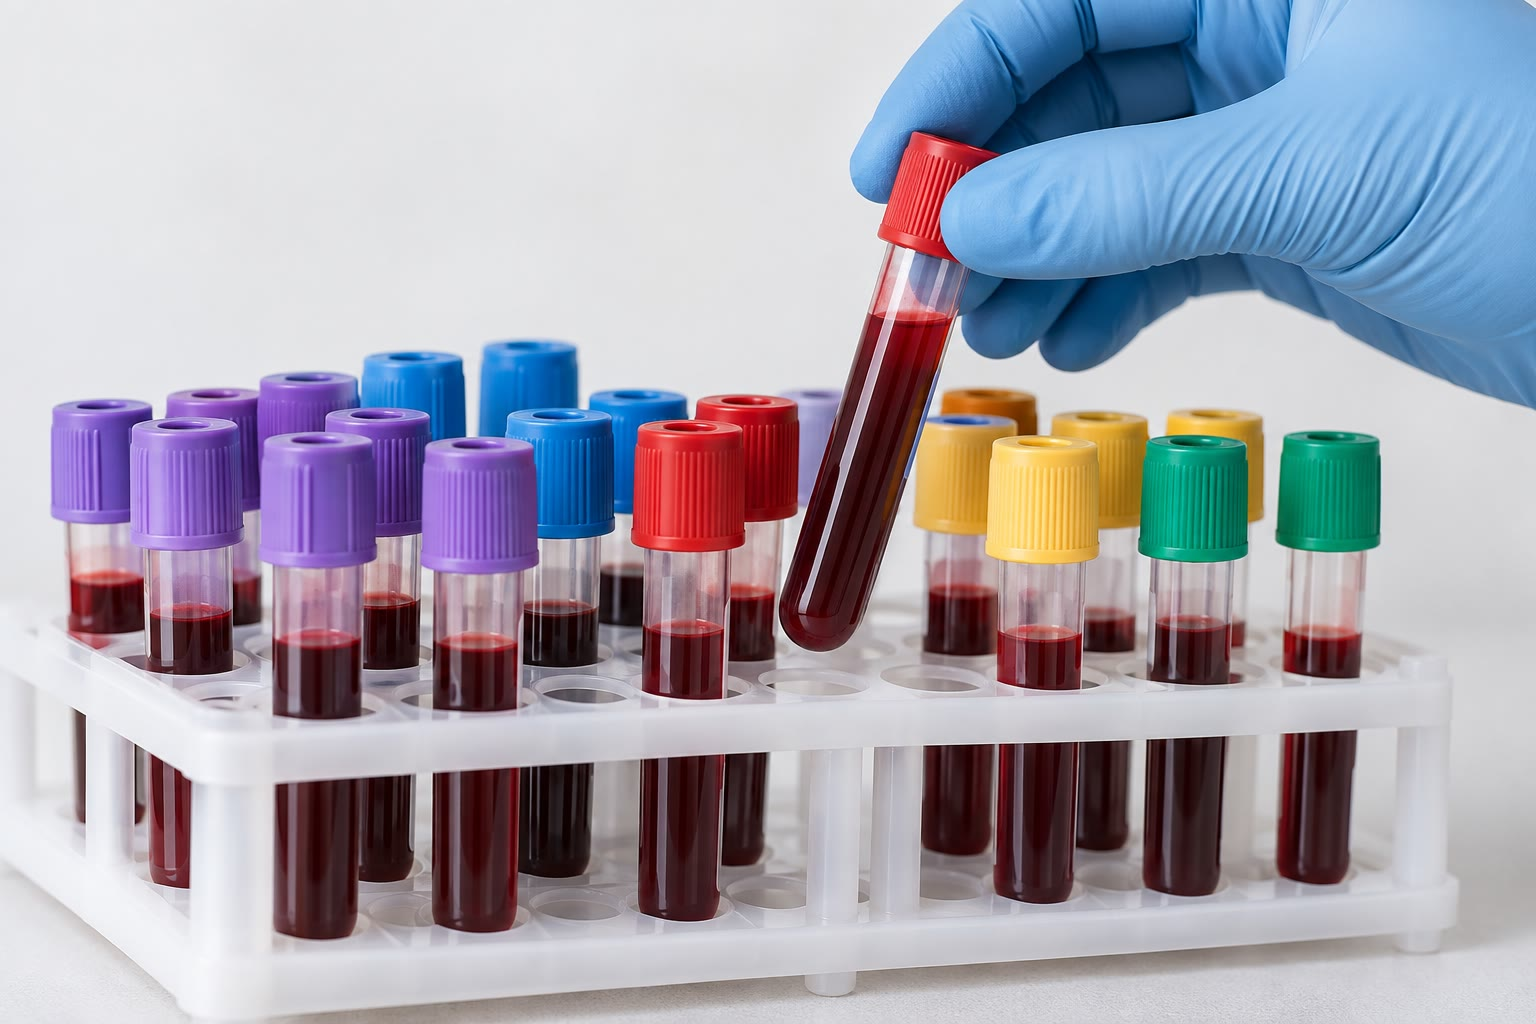
\includegraphics[width=0.45\linewidth]{images/book1/ai/g12-blood-tubes.jpg}

{\small Sampel darah: \omterm{def:g9:acids-bases-ph:ph}{pH-nya} dijaga dalam rentang yang sempit.}
\end{omfigure}

\section{Diagram predominansi}

\begin{proposition}[Hubungan Henderson]\label{prop:g12:buffers-predominance:henderson}
Dalam \omterm{def:g6:solutions-and-solubility:solute}{larutan berair} apa pun yang mengandung pasangan \ce{HA}/\ce{A-},
\[
  \mathrm{pH} = pK_a + \log\frac{[\ce{A-}]}{[\ce{HA}]} .
\]
\end{proposition}

\begin{proof}
Dari $K_a = \dfrac{[\ce{A-}][\ce{H3O+}]}{[\ce{HA}]c^\circ}$, ambillah
$-\log$ kedua ruasnya: $pK_a = \mathrm{pH} - \log\dfrac{[\ce{A-}]}{[\ce{HA}]}$.
\end{proof}

\begin{definition}[Diagram predominansi dan diagram distribusi]\label{def:g12:buffers-predominance:predominance}
Yang disebut \emph{diagram predominansi}\index{diagram predominansi}
sebuah pasangan adalah sumbu \omterm{def:g9:acids-bases-ph:ph}{pH} yang dibagi pada $pK_a$: di bawahnya,
asam HA dominan ($[\ce{HA}] > [\ce{A-}]$), di atasnya, basa \ce{A-}.
Yang disebut \emph{diagram distribusi}\index{diagram distribusi} adalah
diagram yang memperlihatkan fraksi setiap bentuk, $[\ce{HA}]/c$ dan $[\ce{A-}]/c$, terhadap \omterm{def:g9:acids-bases-ph:ph}{pH};
kedua kurvanya berpotongan pada $\mathrm{pH} = pK_a$.
\end{definition}

\begin{method}[Menggambar diagram predominansi]\label{met:g12:buffers-predominance:diagram}
\begin{enumerate}
  \item Gambarlah sumbu \omterm{def:g9:acids-bases-ph:ph}{pH} dari 0 sampai 14 dan tandai $pK_a$ pasangan
        itu.
  \item Tuliskan asamnya di sebelah kiri $pK_a$ dan basanya di sebelah
        kanan.
  \item Untuk spesies dengan beberapa pasangan (asam yang dapat
        melepaskan dua hidrogen, asam amino), tandai setiap $pK_a$:
        setiap selang menjadi milik satu bentuk.
  \item Pada jarak satu satuan dari $pK_a$, perbandingannya sudah 10
        banding 1: bentuk yang minor kurang dari \qty{10}{\percent}.
\end{enumerate}
\end{method}

\begin{omfigure}
\begin{tikzpicture}[font=\small, x=0.62cm]
  % ledger: pka:ethanoic, pka:methanoic, kb:NH3, ka:H2CO3
  \foreach \y/\pk/\acid/\base in {0/3.74/{\ce{HCOOH}}/{\ce{HCOO-}},
      -1.0/4.76/{\ce{CH3COOH}}/{\ce{CH3COO-}}, -2.0/6.37/{\ce{CO2,H2O}}/{\ce{HCO3-}},
      -3.0/9.26/{\ce{NH4+}}/{\ce{NH3}}} {
    \fill[omThm!20] (0,\y) rectangle (\pk,\y+0.5);
    \fill[omDef!20] (\pk,\y) rectangle (14,\y+0.5);
    \draw[black!50] (0,\y) rectangle (14,\y+0.5);
    \node at (\pk/2,\y+0.25) {\acid};
    \node at ({(\pk+14)/2},\y+0.25) {\base};
    \draw[thick] (\pk,\y-0.08) -- (\pk,\y+0.58);
    \node[font=\scriptsize, anchor=south] at (\pk,\y+0.55) {\pk};
  }
  \draw[->] (0,-3.4) -- (14.5,-3.4) node[right] {pH};
  \foreach \k in {0,2,4,6,8,10,12,14} \draw (\k,-3.35) -- (\k,-3.45) node[below, font=\scriptsize] {\k};
\end{tikzpicture}

{\small \omterm{def:g12:buffers-predominance:predominance}{Diagram predominansi} empat pasangan: asam (kiri, merah) dominan
di bawah $pK_a$-nya, basa (kanan, biru) di atasnya.}
\end{omfigure}

\begin{omfigure}
\begin{minipage}{0.49\linewidth}
\begin{tikzpicture}
\begin{axis}[width=\linewidth, height=5cm, xmin=0, xmax=14, ymin=0, ymax=1.05,
    xlabel={pH}, ylabel={fraksi}, axis lines*=left, ymajorgrids,
    grid style={gray!20}, tick label style={font=\scriptsize},
    label style={font=\small}, title={\small asam etanoat},
    title style={yshift=-4pt}]
  \addplot[very thick, omThm] table[x=pH, y=HA] {figdata/out/grade-12-buffers-predominance-a.dat};
  \addplot[very thick, omDef] table[x=pH, y=A] {figdata/out/grade-12-buffers-predominance-a.dat};
  \addplot[dashed, black!50] coordinates {(4.76,0) (4.76,1)};
  \node[font=\scriptsize, omThm] at (axis cs:2.2,0.85) {\ce{CH3COOH}};
  \node[font=\scriptsize, omDef] at (axis cs:7.6,0.85) {\ce{CH3COO-}};
\end{axis}
\end{tikzpicture}
\end{minipage}\hfill
\begin{minipage}{0.49\linewidth}
\begin{tikzpicture}
\begin{axis}[width=\linewidth, height=5cm, xmin=0, xmax=14, ymin=0, ymax=1.05,
    xlabel={pH}, ylabel={fraksi}, axis lines*=left, ymajorgrids,
    grid style={gray!20}, tick label style={font=\scriptsize},
    label style={font=\small}, title={\small glisina},
    title style={yshift=-4pt}]
  \addplot[very thick, omThm] table[x=pH, y=cation] {figdata/out/grade-12-buffers-predominance-b.dat};
  \addplot[very thick, omMeth] table[x=pH, y=zwitterion] {figdata/out/grade-12-buffers-predominance-b.dat};
  \addplot[very thick, omDef] table[x=pH, y=anion] {figdata/out/grade-12-buffers-predominance-b.dat};
  \node[font=\scriptsize, omThm] at (axis cs:1.0,0.55) {kation};
  \node[font=\scriptsize, omMeth] at (axis cs:6.1,0.88) {ion zwitter};
  \node[font=\scriptsize, omDef] at (axis cs:12.6,0.55) {anion};
\end{axis}
\end{tikzpicture}
\end{minipage}

{\small \omterm{def:g12:buffers-predominance:predominance}{Diagram distribusi}, yang dihitung dari nilai-nilai $pK_a$. Kiri:
asam etanoat, kurvanya berpotongan pada 4.76. Kanan: glisina,
\ce{H2N-CH2-COOH}, dengan dua pasangan ($pK_a$ 2.35 dan 9.78): \omterm{def:g9:ions:ion}{kation}
\ce{H3N+-CH2-COOH}, \omterm{def:g9:ions:ion}{ion} zwitter \ce{H3N+-CH2-COO-}, dan \omterm{def:g9:ions:ion}{anion}
\ce{H2N-CH2-COO-}.}
\end{omfigure}

\begin{example}[Glisina di dalam tubuh]\label{ex:g12:buffers-predominance:glycine}
% ledger: pka:glycine1, pka:glycine2, ph:blood
Pada \omterm{def:g9:acids-bases-ph:ph}{pH} darah, sekitar 7.4, glisina berada di antara kedua nilai
$pK_a$-nya: glisina hampir seluruhnya berbentuk \omterm{def:g9:ions:ion}{ion} zwitter, yang
bermuatan positif pada nitrogennya dan bermuatan negatif pada gugus
karboksilatnya, netral secara keseluruhan. Setiap asam amino berperilaku
dengan cara yang sama.
\end{example}

\section{Indikator asam--basa}


\begin{definition}[Indikator asam--basa, trayek perubahan warna]\label{def:g12:buffers-predominance:indicator}
Yang disebut \emph{indikator asam--basa}\index{indikator asam--basa}
adalah pasangan \ce{HInd}/\ce{Ind-} yang kedua bentuknya berbeda
warna, yang dipakai dalam jumlah yang sangat kecil.
Yang disebut \emph{trayek perubahan warna}\index{trayek perubahan warna}
indikator itu adalah selang \omterm{def:g9:acids-bases-ph:ph}{pH} tempat warnanya terlihat berubah, kira-kira dari $pK_a - 1$
sampai $pK_a + 1$: di bawahnya, warna \ce{HInd} yang terlihat, di
atasnya, warna \ce{Ind-}, dan di antaranya \omterm{def:g6:pure-substances-and-mixtures:mixture}{campuran} keduanya.
\end{definition}

\begin{omfigure}
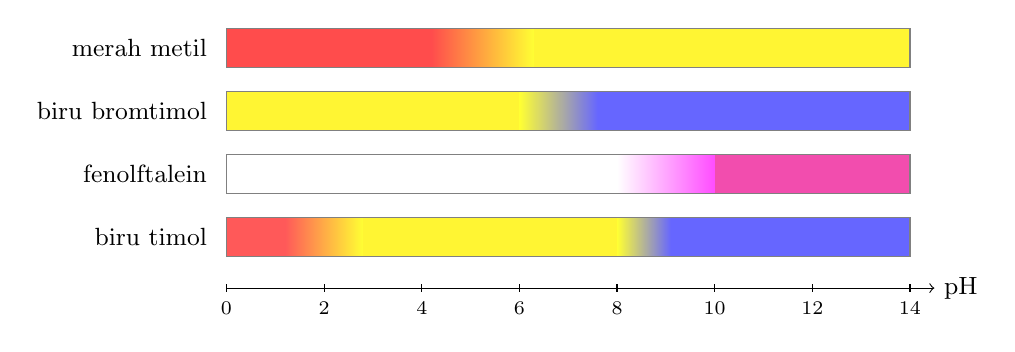
\begin{tikzpicture}[font=\small, x=0.62cm]
  % ledger: ind:methyl-red, ind:BBT, ind:phenolphthalein, ind:thymol-blue, ind:range-rule
  \foreach \y/\name/\a/\b/\ca/\cm/\cb in {
      0/{merah metil}/4.2/6.3/red!70/orange/yellow!80,
      -0.8/{biru bromtimol}/6.0/7.6/yellow!80/green!60/blue!60,
      -1.6/{fenolftalein}/8.0/10.0/white/magenta!25/magenta!70} {
    \fill[\ca] (0,\y) rectangle (\a,\y+0.5);
    \shade[left color=\ca, right color=\cb] (\a,\y) rectangle (\b,\y+0.5);
    \fill[\cb] (\b,\y) rectangle (14,\y+0.5);
    \draw[black!50] (0,\y) rectangle (14,\y+0.5);
    \node[anchor=east] at (-0.2,\y+0.25) {\name};
  }
  \fill[red!65] (0,-2.4) rectangle (1.2,-1.9);
  \shade[left color=red!65, right color=yellow!80] (1.2,-2.4) rectangle (2.8,-1.9);
  \fill[yellow!80] (2.8,-2.4) rectangle (8.0,-1.9);
  \shade[left color=yellow!80, right color=blue!60] (8.0,-2.4) rectangle (9.1,-1.9);
  \fill[blue!60] (9.1,-2.4) rectangle (14,-1.9);
  \draw[black!50] (0,-2.4) rectangle (14,-1.9);
  \node[anchor=east] at (-0.2,-2.15) {biru timol};
  \draw[->] (0,-2.8) -- (14.5,-2.8) node[right] {pH};
  \foreach \k in {0,2,4,6,8,10,12,14} \draw (\k,-2.75) -- (\k,-2.85) node[below, font=\scriptsize] {\k};
\end{tikzpicture}

{\small Warna empat indikator terhadap \omterm{def:g9:acids-bases-ph:ph}{pH}; bagian yang diarsir adalah
\omterm{def:g12:buffers-predominance:indicator}{trayek perubahan warnanya}. Biru timol, dengan dua pasangan, memiliki dua
trayek.}
\end{omfigure}

\begin{method}[Memilih indikator]\label{met:g12:buffers-predominance:indicator}
Untuk mendeteksi kapan sebuah larutan melewati \omterm{def:g9:acids-bases-ph:ph}{pH} tertentu (misalnya \omterm{def:g9:acids-bases-ph:ph}{pH}
pada akhir \omterm{def:g11:titration:titration}{titrasi}), pilihlah indikator yang \omterm{def:g12:buffers-predominance:indicator}{trayek perubahan warnanya}
mencakup \omterm{def:g9:acids-bases-ph:ph}{pH} itu: warnanya lalu berubah tepat di sana.
\end{method}

\section{Larutan penyangga}

\begin{definition}[Larutan penyangga]\label{def:g12:buffers-predominance:buffer}
Yang disebut \emph{larutan penyangga}\index{larutan penyangga} adalah
larutan yang \omterm{def:g9:acids-bases-ph:ph}{pH-nya} sangat sedikit berubah jika sedikit asam atau basa
ditambahkan, atau jika larutan itu diencerkan. Larutan ini biasanya
dibuat dari \omterm{def:g12:ka-and-pka:strong-acid}{asam lemah} dan basa konjugatnya dalam jumlah yang sebanding;
\omterm{def:g9:acids-bases-ph:ph}{pH-nya} lalu dekat dengan $pK_a$ pasangan itu.
\end{definition}

\begin{proposition}[Mengapa penyangga bertahan]\label{prop:g12:buffers-predominance:buffer}
Dalam penyangga \ce{HA} dan \ce{A-}, \omterm{def:g12:ka-and-pka:strong-acid}{asam kuat} yang ditambahkan dihabiskan
oleh \ce{A-} (\ce{A- + H3O+ -> HA + H2O}) dan \omterm{def:g12:ka-and-pka:strong-acid}{basa kuat} yang ditambahkan
oleh \ce{HA} (\ce{HA + OH- -> A- + H2O}); perbandingan
$[\ce{A-}]/[\ce{HA}]$, dan karena itu \omterm{def:g9:acids-bases-ph:ph}{pH-nya}, hanya sedikit berubah.
\omterm{def:g10:concentration-and-dilution:dilution}{Pengenceran} sama sekali tidak mengubah perbandingan itu.
\end{proposition}

\begin{proof}
Menurut hubungan Henderson, \omterm{def:g9:acids-bases-ph:ph}{pH} hanya bergantung pada perbandingan itu.
Menambahkan \qty{1}{mmol} asam pada penyangga yang mengandung
\qty{10}{mmol} setiap bentuk mengubah perbandingannya dari $10/10$
menjadi $9/11$, dan \omterm{def:g9:acids-bases-ph:ph}{pH-nya} hanya sebesar $\log(9/11) = -0.09$.
\end{proof}

\begin{omfigure}
\begin{tikzpicture}
\begin{axis}[width=0.75\linewidth, height=5.6cm, xmin=0, xmax=10, ymin=0,
    ymax=8, xlabel={\ce{HCl} \qty{0.10}{mol/L} yang ditambahkan (\si{mL})},
    ylabel={pH}, axis lines*=left, ymajorgrids, grid style={gray!20},
    tick label style={font=\small}, label style={font=\small},
    legend style={font=\small, at={(0.98,0.97)}, anchor=north east,
    draw=none, fill=white}, legend cell align=left]
  % ledger: pka:ethanoic (buffer recipe: exercise data)
  \addplot[very thick, omThm, mark=*, mark size=1.3pt] table[x=V, y=water]
    {figdata/out/grade-12-buffers-predominance-c.dat};
  \addplot[very thick, omDef, mark=*, mark size=1.3pt] table[x=V, y=buffer]
    {figdata/out/grade-12-buffers-predominance-c.dat};
  \legend{\qty{100}{mL} air murni, \qty{100}{mL} penyangga etanoat}
\end{axis}
\end{tikzpicture}

{\small Penambahan asam klorida pada air murni dan pada penyangga asam
etanoat dan natrium etanoat (masing-masing \qty{0.10}{mol/L}). \omterm{def:g9:acids-bases-ph:ph}{pH} air
turun dari 7 menjadi sekitar 2; \omterm{def:g9:acids-bases-ph:ph}{pH} penyangga dari 4.76 menjadi 4.67.}
\end{omfigure}

\begin{method}[Menyiapkan larutan penyangga]\label{met:g12:buffers-predominance:prepare}
\begin{enumerate}
  \item Pilihlah pasangan yang $pK_a$-nya berjarak paling jauh satu
        satuan dari \omterm{def:g9:acids-bases-ph:ph}{pH} yang diinginkan (idealnya dekat dengannya).
  \item Hitung perbandingan $[\ce{A-}]/[\ce{HA}] = 10^{\mathrm{pH} - pK_a}$.
  \item \omterm{def:g2:mixing-and-dissolving:mix}{Campurkan} \omterm{def:g12:ka-and-pka:strong-acid}{asam lemah} dan garam basanya dengan perbandingan itu,
        pada konsentrasi yang cukup tinggi agar jumlah asam atau basa
        yang ditambahkan dapat diredam.
\end{enumerate}
\end{method}

\begin{inthelab}[Menyiapkan penyangga pH 4.8]
Sebanyak \qty{50.0}{mL} asam etanoat \qty{0.10}{mol/L} \omterm{def:g2:mixing-and-dissolving:mix}{dicampur} dengan
\qty{50.0}{mL} natrium etanoat \qty{0.10}{mol/L}; \omterm{def:g9:acids-bases-ph:ph-paper}{pH meter} menunjukkan
sekitar 4.8. Beberapa tetes asam klorida \qty{1}{mol/L} hampir tidak
menggeser angkanya, sedangkan tetes-tetes yang sama dalam \qty{100}{mL}
air suling menurunkannya sampai sekitar 3.
\end{inthelab}

\section{Penyangga pada makhluk hidup}

\begin{example}[Penyangga darah]\label{ex:g12:buffers-predominance:blood}
% ledger: pk:blood-bicarb, ph:blood, hco3:blood
Penyangga utama darah adalah pasangan karbon dioksida terlarut dan \omterm{def:g9:ions:ion}{ion}
hidrogenkarbonat, \ce{CO2,H2O}/\ce{HCO3-}. Untuk darah, para ahli
fisiologi memakai hubungan $\mathrm{pH} = 6.1 +
\log\big([\ce{HCO3-}]/[\ce{CO2}]\big)$. Paru-paru mengeluarkan karbon
dioksida, ginjal mengatur hidrogenkarbonat: bersama-sama keduanya
menjaga perbandingan itu, dan karena itu \omterm{def:g9:acids-bases-ph:ph}{pH-nya}.
\end{example}

\begin{omfigure}
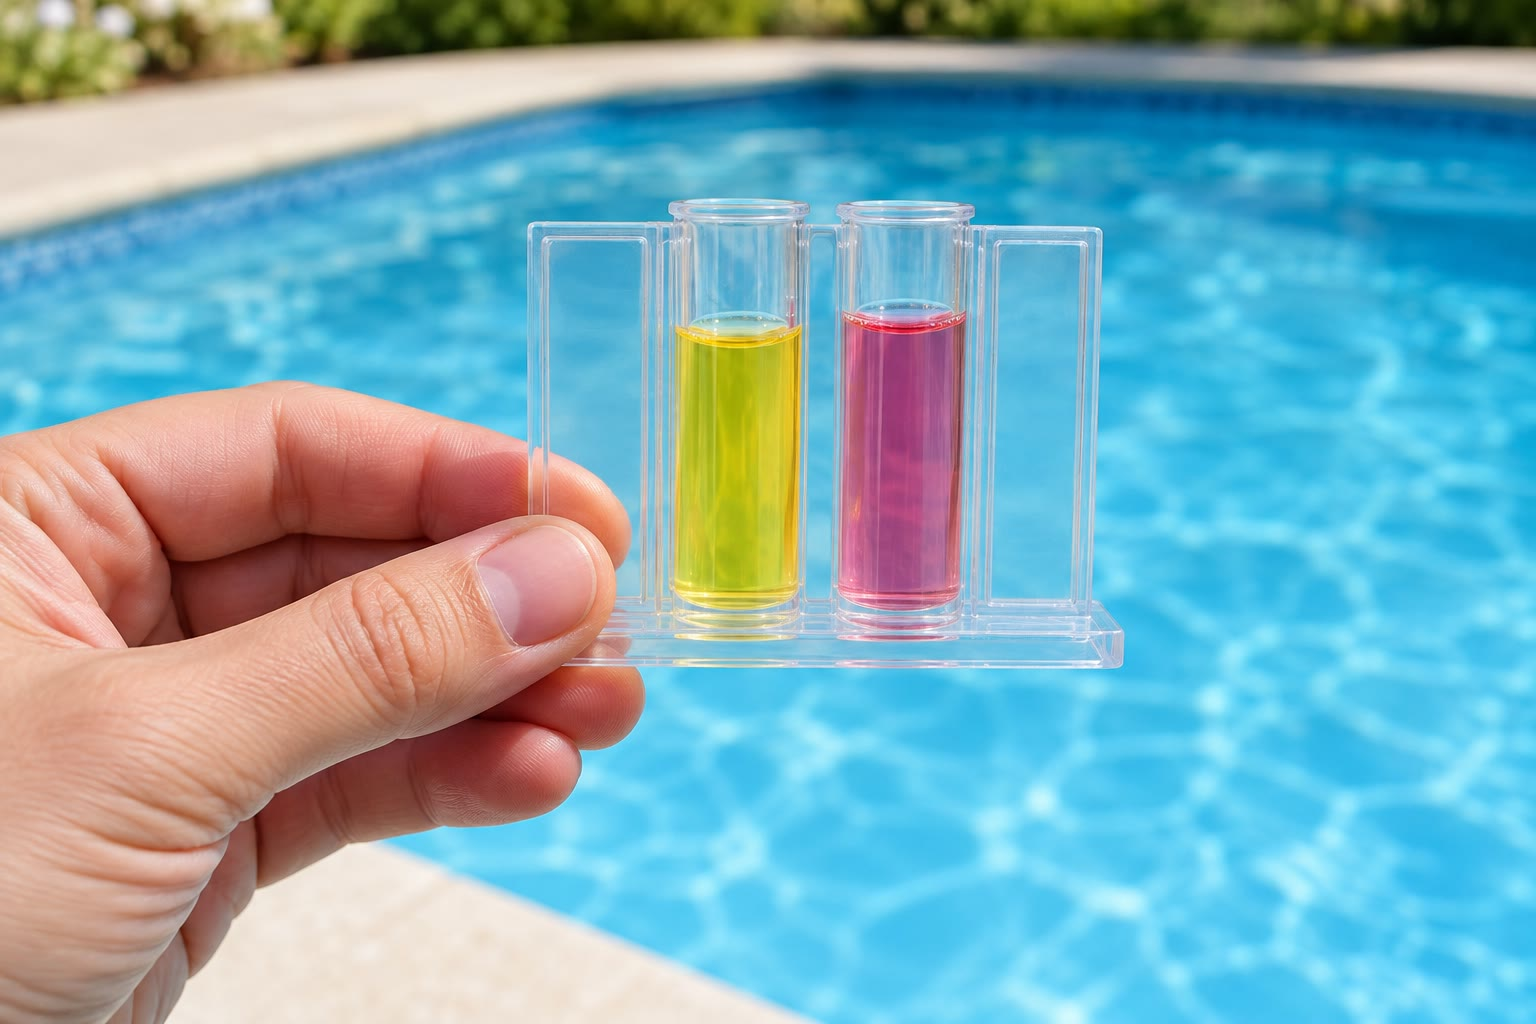
\includegraphics[width=0.45\linewidth]{images/book1/ai/g12-pool-test.jpg}

{\small Menguji air kolam renang: warna indikator memberikan \omterm{def:g9:acids-bases-ph:ph}{pH-nya}.}
\end{omfigure}

\section{Latihan}


\begin{exercise}[$\star$]\label{exo:g12:buffers-predominance:1}
Bentuk mana dari pasangan \ce{CH3COOH}/\ce{CH3COO-} ($pK_a = 4.76$)
yang dominan pada \omterm{def:g9:acids-bases-ph:ph}{pH} 2, pada \omterm{def:g9:acids-bases-ph:ph}{pH} 4.76, dan pada \omterm{def:g9:acids-bases-ph:ph}{pH} 7?
\end{exercise}

\begin{exercise}[$\star$]\label{exo:g12:buffers-predominance:2}
Pada \omterm{def:g12:buffers-predominance:predominance}{diagram distribusi} asam etanoat, bacalah fraksi \ce{CH3COO-} pada
\omterm{def:g9:acids-bases-ph:ph}{pH} 4 dan pada \omterm{def:g9:acids-bases-ph:ph}{pH} 6.
\end{exercise}

\begin{exercise}[$\star$]\label{exo:g12:buffers-predominance:3}
Apa warna biru bromtimol pada \omterm{def:g9:acids-bases-ph:ph}{pH} 5? Pada \omterm{def:g9:acids-bases-ph:ph}{pH} 7? Pada \omterm{def:g9:acids-bases-ph:ph}{pH} 9?
\end{exercise}

\begin{exercise}[$\star$]\label{exo:g12:buffers-predominance:4}
Bentuk mana dari pasangan \ce{NH4+}/\ce{NH3} yang dominan dalam larutan
\omterm{def:g9:acids-bases-ph:ph}{ber-pH} 7.4? Pada \omterm{def:g9:acids-bases-ph:ph}{pH} 11?
\end{exercise}

\begin{exercise}[$\star$]\label{exo:g12:buffers-predominance:5}
Mengapa indikator dipakai dalam jumlah yang sangat kecil?
\end{exercise}

\begin{exercise}[$\star\star$]\label{exo:g12:buffers-predominance:6}
Hitung perbandingan $[\ce{CH3COO-}]/[\ce{CH3COOH}]$ pada \omterm{def:g9:acids-bases-ph:ph}{pH} 3.76, 4.76,
dan 5.76.
\end{exercise}

\begin{exercise}[$\star\star$]\label{exo:g12:buffers-predominance:7}
Sebuah \omterm{def:g11:titration:titration}{titrasi} berakhir pada \omterm{def:g9:acids-bases-ph:ph}{pH} 8.7. Indikator mana dari keempat
indikator dalam gambar yang akan kamu pilih? Mengapa bukan merah metil?
\end{exercise}

\begin{exercise}[$\star\star$]\label{exo:g12:buffers-predominance:8}
Sebuah penyangga mengandung \qty{0.20}{mol/L} asam etanoat dan
\qty{0.10}{mol/L} natrium etanoat. Hitung \omterm{def:g9:acids-bases-ph:ph}{pH-nya}.
\end{exercise}

\begin{exercise}[$\star\star$]\label{exo:g12:buffers-predominance:9}
Dengan diagram glisina, sebutkan bentuk yang dominan pada \omterm{def:g9:acids-bases-ph:ph}{pH} 1, 6, dan
12, beserta muatannya.
\end{exercise}

\begin{exercise}[$\star\star$]\label{exo:g12:buffers-predominance:10}
Bacalah kurva tanggapannya: berapa penurunan \omterm{def:g9:acids-bases-ph:ph}{pH} air setelah ditambah
\qty{1.0}{mL} asam? Dan \omterm{def:g9:acids-bases-ph:ph}{pH} penyangga?
\end{exercise}

\begin{exercise}[$\star\star$]\label{exo:g12:buffers-predominance:11}
Pasangan mana dalam gambar predominansi yang akan kamu pilih untuk
membuat penyangga \omterm{def:g9:acids-bases-ph:ph}{pH} 9.5? Dengan perbandingan berapa kamu akan \omterm{def:g2:mixing-and-dissolving:mix}{mencampur}
kedua bentuknya?
\end{exercise}

\begin{exercise}[$\star\star\star$]\label{exo:g12:buffers-predominance:12}
Penyangga etanoat dalam gambar (\qty{10}{mmol} setiap bentuk) menerima
asam klorida. Berapa banyak asam yang dapat diterimanya sebelum \omterm{def:g9:acids-bases-ph:ph}{pH-nya}
turun satu satuan? Mengapa penyangga yang lebih pekat dikatakan memiliki
kapasitas yang lebih besar?
\end{exercise}

\begin{exercise}[$\star\star\star$]\label{exo:g12:buffers-predominance:13}
Berapa volume larutan natrium etanoat \qty{0.10}{mol/L} yang harus
ditambahkan pada \qty{100}{mL} asam etanoat \qty{0.10}{mol/L} untuk
memperoleh penyangga \omterm{def:g9:acids-bases-ph:ph}{pH} 5.0?
\end{exercise}

\begin{exercise}[$\star\star\star$]\label{exo:g12:buffers-predominance:14}
Biru timol memiliki dua \omterm{def:g12:buffers-predominance:indicator}{trayek perubahan warna}. Jelaskan mengapa, lalu
sebutkan warnanya pada \omterm{def:g9:acids-bases-ph:ph}{pH} 1, 5, dan 10.
\end{exercise}

\begin{exercise}[$\star\star\star$]\label{exo:g12:buffers-predominance:15}
Penyangga \omterm{def:g9:acids-bases-ph:ph}{pH} 4.76 diencerkan sepuluh kali dengan air suling. Berapa
\omterm{def:g9:acids-bases-ph:ph}{pH-nya} yang baru, menurut hubungan Henderson? Apa yang terjadi jika \omterm{def:g12:ka-and-pka:strong-acid}{asam
kuat} dengan \omterm{def:g9:acids-bases-ph:ph}{pH} yang sama diencerkan sepuluh kali?
\end{exercise}

\section{Soal: Penyangga Darah}

\begin{problem}[{Soal akhir pekan --- berapa perbandingan
hidrogenkarbonat terhadap karbon dioksida yang menjaga darah pada pH
7.4?}]
\label{pb:g12:buffers-predominance:1}
% ledger: pk:blood-bicarb, ph:blood, hco3:blood
\omterm{def:g9:acids-bases-ph:ph}{pH} darah arteri normalnya antara 7.38 dan 7.42. Penyangga utamanya
adalah pasangan \ce{CO2,H2O}/\ce{HCO3-}, yang untuknya para ahli
fisiologi memakai $\mathrm{pH} = 6.1 + \log\big([\ce{HCO3-}]/[\ce{CO2}]\big)$.
Konsentrasi hidrogenkarbonat darah yang normal adalah 22 sampai
\qty{28}{mmol/L}.

\medskip
\noindent\textbf{Bagian I --- Pasangannya.}
\begin{enumerate}
  \item Tuliskan reaksi karbon dioksida terlarut dengan air yang
        menghasilkan \omterm{def:g9:ions:ion}{ion} hidrogenkarbonat.
  \item Spesies mana yang menjadi asam, mana yang menjadi basa?
  \item Nilai 6.1 berbeda dari 6.37 pada tabel $pK_a$. Berikan sebuah
        alasan (pikirkan suhu tubuh dan \omterm{def:g9:ions:ion}{ion-ion} lain yang ada).
  \item Berapa jumlah hidrogenkarbonat yang dikandung \qty{5.0}{L} darah
        pada \qty{24}{mmol/L}?
\end{enumerate}

\medskip
\noindent\textbf{Bagian II --- Predominansi.}
\begin{enumerate}[resume]
  \item Gambarlah \omterm{def:g12:buffers-predominance:predominance}{diagram predominansi} pasangan itu dengan $pK = 6.1$.
  \item Bentuk mana yang dominan dalam darah?
  \item Apakah darah sedikit asam atau sedikit basa?
\end{enumerate}

\medskip
\noindent\textbf{Bagian III --- Perbandingannya.}
\begin{enumerate}[resume]
  \item Dengan hubungan itu, hitung perbandingan $[\ce{HCO3-}]/[\ce{CO2}]$
        pada \omterm{def:g9:acids-bases-ph:ph}{pH} 7.4.
  \item Dengan $[\ce{HCO3-}] = \qty{24}{mmol/L}$, hitung $[\ce{CO2}]$.
  \item Hitung perbandingannya pada kedua ujung rentang normal, 7.38 dan
        7.42.
  \item Berapa bagian pasangan itu yang berbentuk hidrogenkarbonat pada
        \omterm{def:g9:acids-bases-ph:ph}{pH} 7.4?
  \item Darah yang terlalu basa dapat mencapai \omterm{def:g9:acids-bases-ph:ph}{pH} 7.6. Berapa
        perbandingannya saat itu?
\end{enumerate}

\medskip
\noindent\textbf{Bagian IV --- Ketika keseimbangan hilang.}
\begin{enumerate}[resume]
  \item Selama aktivitas berat, asam-asam masuk ke dalam darah. Bentuk
        mana dari pasangan itu yang menghabiskannya? Tuliskan reaksinya.
  \item Jika \omterm{def:g9:acids-bases-ph:ph}{pH} turun sampai 7.1, menjadi berapa perbandingannya?
  \item Dengan hidrogenkarbonat yang tidak berubah, berapa banyak karbon
        dioksida harus bertambah? Apa yang dilakukan paru-paru untuk
        melawannya?
  \item Mengapa \omterm{def:g12:ka-and-pka:strong-acid}{asam lemah} beserta basanya, dan bukan \omterm{def:g12:ka-and-pka:strong-acid}{asam kuat}, yang
        menjadi alat yang tepat untuk menjaga \omterm{def:g9:acids-bases-ph:ph}{pH}?
  \item Berapa perubahan \omterm{def:g9:acids-bases-ph:ph}{pH} jika kedua konsentrasi dibagi dua? Mengapa?
  \item Nyatakan jawaban akhirnya: berapa perbandingan hidrogenkarbonat
        terhadap karbon dioksida dalam darah pada \omterm{def:g9:acids-bases-ph:ph}{pH} 7.4?
\end{enumerate}
\end{problem}
